\documentclass[11pt, a4paper]{article}
\usepackage{pdfpages}
\usepackage{parallel}
\usepackage[T2A]{fontenc}
%\usepackage{ucs}
\usepackage[utf8]{inputenc}
\usepackage[english,russian]{babel}
\usepackage{hyperref}
\usepackage{rotating}
\usepackage[inner=2cm,top=1.8cm,outer=2cm,bottom=2.3cm,nohead]{geometry}
%\usepackage{listings}
\usepackage{graphicx}
\usepackage{wrapfig}
\usepackage{longtable}
\usepackage{indentfirst}
\usepackage{array}
\usepackage{tikzsymbols}
\usepackage{soul}
\usepackage[ruled,vlined]{algorithm2e}
\usepackage{qrcode}
\counterwithout{figure}{section} 

\usepackage{url}
\makeatletter
\g@addto@macro{\UrlBreaks}{\UrlOrds}
\makeatother

\newcolumntype{P}[1]{>{\raggedright\arraybackslash}p{#1}}
\frenchspacing
%\usepackage{fixltx2e} %text sub- and superscripts
\usepackage{icomma} % коскі ў матэматычным рэжыме
%\PreloadUnicodePage{4}

\newcommand{\longpage}{\enlargethispage{\baselineskip}}
\newcommand{\shortpage}{\enlargethispage{-\baselineskip}}

\def\switchlang#1{\expandafter\csname switchlang#1\endcsname}
\def\switchlangbe{
\let\saverefname=\refname%
\def\refname{Літаратура}%
\def\figurename{Іл.}%
}
\def\switchlangru{
\let\saverefname=\refname%
\let\savefigurename=\figurename%
\def\refname{Литература}%
\def\figurename{Рис.}%
}
\def\switchlangen{
\let\saverefname=\refname%
\def\refname{References}%
\def\figurename{Fig.}%
}

\hyphenation{admi-ni-stra-tive}
\hyphenation{ex-pe-ri-ence}
\hyphenation{fle-xi-bi-li-ty}
\hyphenation{Py-thon}
\hyphenation{ma-the-ma-ti-cal}
\hyphenation{re-ported}
\hyphenation{imp-le-menta-tions}
\hyphenation{pro-vides}
\hyphenation{en-gi-neering}
\hyphenation{com-pa-ti-bi-li-ty}
\hyphenation{im-pos-sible}
\hyphenation{desk-top}
\hyphenation{elec-tro-nic}
\hyphenation{com-pa-ny}
\hyphenation{de-ve-lop-ment}
\hyphenation{de-ve-loping}
\hyphenation{de-ve-lop}
\hyphenation{da-ta-ba-se}
\hyphenation{plat-forms}
\hyphenation{or-ga-ni-za-tion}
\hyphenation{pro-gramming}
\hyphenation{in-stru-ments}
\hyphenation{Li-nux}
\hyphenation{sour-ce}
\hyphenation{en-vi-ron-ment}
\hyphenation{Te-le-pathy}
\hyphenation{Li-nux-ov-ka}
\hyphenation{Open-BSD}
\hyphenation{Free-BSD}
\hyphenation{men-ti-on-ed}
\hyphenation{app-li-ca-tion}

\def\progref!#1!{\texttt{#1}}
\renewcommand{\arraystretch}{2} %Іначай формулы ў матрыцы зліпаюцца з лініямі
\usepackage{array}

\def\interview #1 (#2), #3, #4, #5\par{

\section[#1, #3, #4]{#1 -- #3, #4}
\def\qname{LVEE}
\def\aname{#1}
\def\q ##1\par{{\noindent \bf \qname: ##1 }\par}
\def\a{{\noindent \bf \aname: } \def\qname{L}\def\aname{#2}}
}

\def\interview* #1 (#2), #3, #4, #5\par{

\section*{#1\\{\small\rm #3, #4. #5}}
\ifx\ParallelWhichBox\undefined%
    \addcontentsline{toc}{section}{#1, #3, #4}%
\else%
\ifnum\ParallelWhichBox=0%
    \addcontentsline{toc}{section}{#1, #3, #4}%
\fi\fi%

\def\qname{LVEE}
\def\aname{#1}
\def\q ##1\par{{\noindent \bf \qname: ##1 }\par}
\def\a{{\noindent \bf \aname: } \def\qname{L}\def\aname{#2}}
}

\newcommand{\interviewfooter}[1]{
\vskip 1em
\noindent \textit{#1}
}

\AtEndDocument{\vfill\centering \qrcode{https://github.com/fiowro/mouses/blob/main/\jobname.pdf}}

\switchlang{ru}
\begin{document}

\title{1985 "--- SMC/Contriver Magic Mouse}
\date{}
\maketitle
\selectlanguage{russian}

Мышь Magic Mouse появилась на рынке в 1985 году. Она продавалась под этим именем в версиях для компьютеров Commodore 64 и BBC Micro. Аналогичная модель для компьютеров Apple II, отличающаяся цветом клавиш и разъёмом подключения, продавалась под названием Graphic Mouse \cite{SMC_Mouse_Commodore1}. В обзорах в качестве производителя Magic Mouse обычно указывают либо компанию SMC Supplies \cite{c64wiki, SMC_Mouse_Commodore3}, либо Connexions \cite{SMC_Mouse_Commodore2}. Однако Magic Mouse является первой мышью в линейке мышей Contriver, вопреки путанице с названием и производителем, отчасти характерной для этой линейки \cite{reddit}. Упаковка Graphic mouse для Apple II не содержит информации о производителе, а упаковка мыши в варианте для Commodore 64 демонстрирует название <<Ideal Magic Mouse>> (либо просто Magic Mouse --- первое слово отличается оформлением и может быть  эмблемой), рекламный вкладыш от Graphic Mouse и, наконец, указание Contriver в качестве  производителя \cite{CHM}.

\begin{figure}[h]
   \centering
    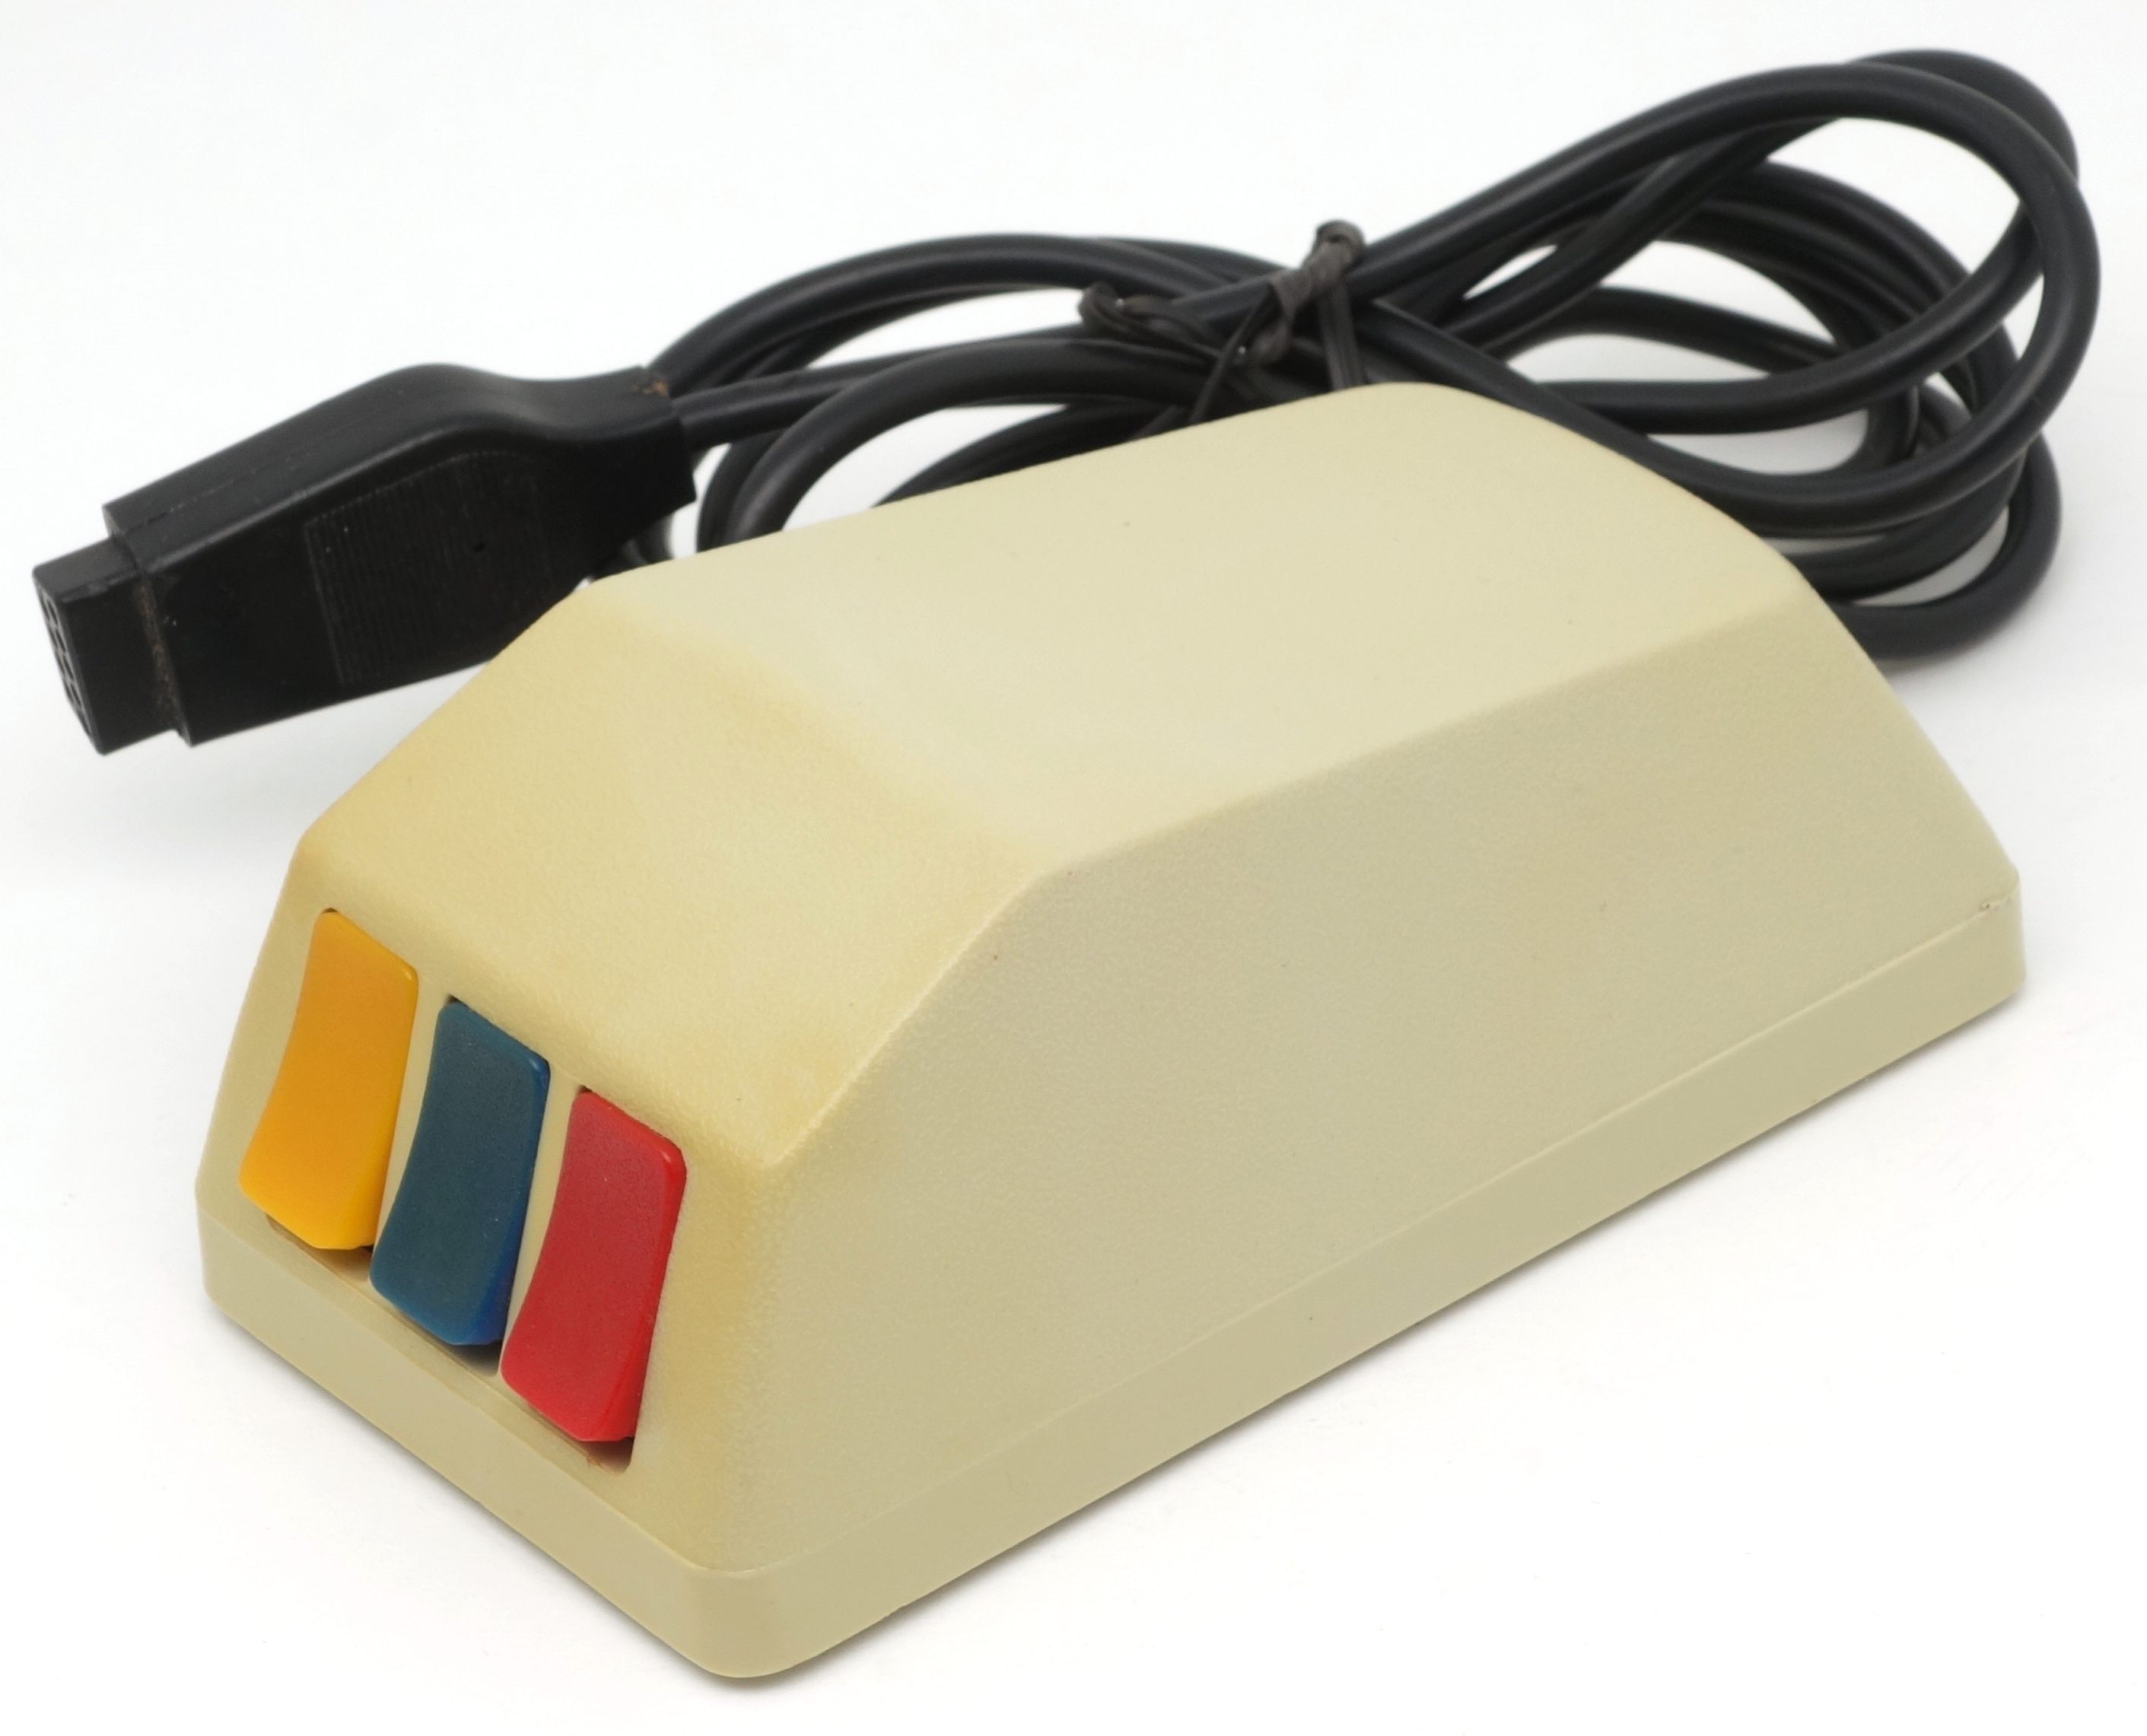
\includegraphics[scale=0.6]{1985_smc_contriver_magic_mouse/pic_30.jpg}
    \caption{Magic Mouse}
    \label{fig:MagicMousePic}
\end{figure}

Мышь выполнена в бежевом корпусе рубленых очертаний и имеет три цветные кнопки на наклонной передней (то есть дальней от пользователя) стороне --- красной, синей и желтой (рис. \ref{fig:MagicMousePic}). Толстый провод  выходит с правой стороны корпуса и имеет муфту для защиты от механических повреждений в месте выхода. На нижней стороне (рис. \ref{fig:MagicMouseTopAndBottom}) присутствует крупный резиновый шар, расположенный вплотную к задней части корпуса, съемное кольцо, позволяющее извлечь его для чистки мыши (оно крепится шурупом --- конструкция, характерная для мышей первой половины 80-х годов), а также два регулировочных винта. С помощью винтов выполняется калибровка, чтобы указатель мог перемещаться по всему экрану: мышь подключается к порту аналогового джойстика и фактически его эмулирует, а винты играют роль триммеров джойстика.

\begin{figure}[h]
    \centering
    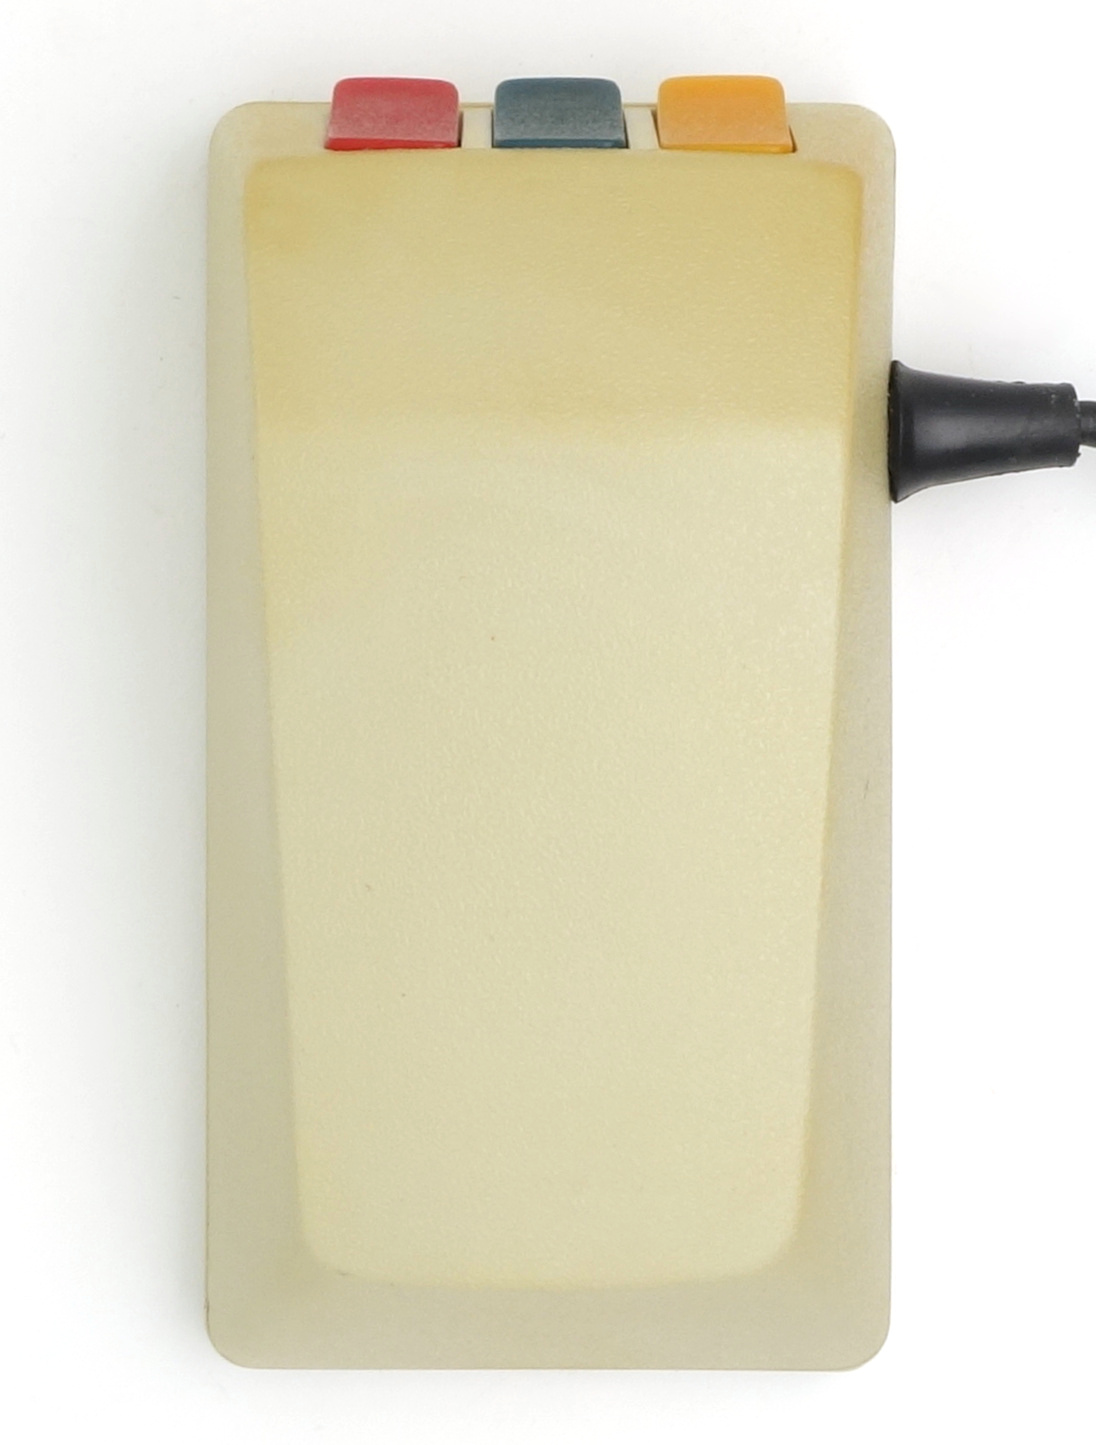
\includegraphics[scale=0.75]{1985_smc_contriver_magic_mouse/top_30.jpg}
    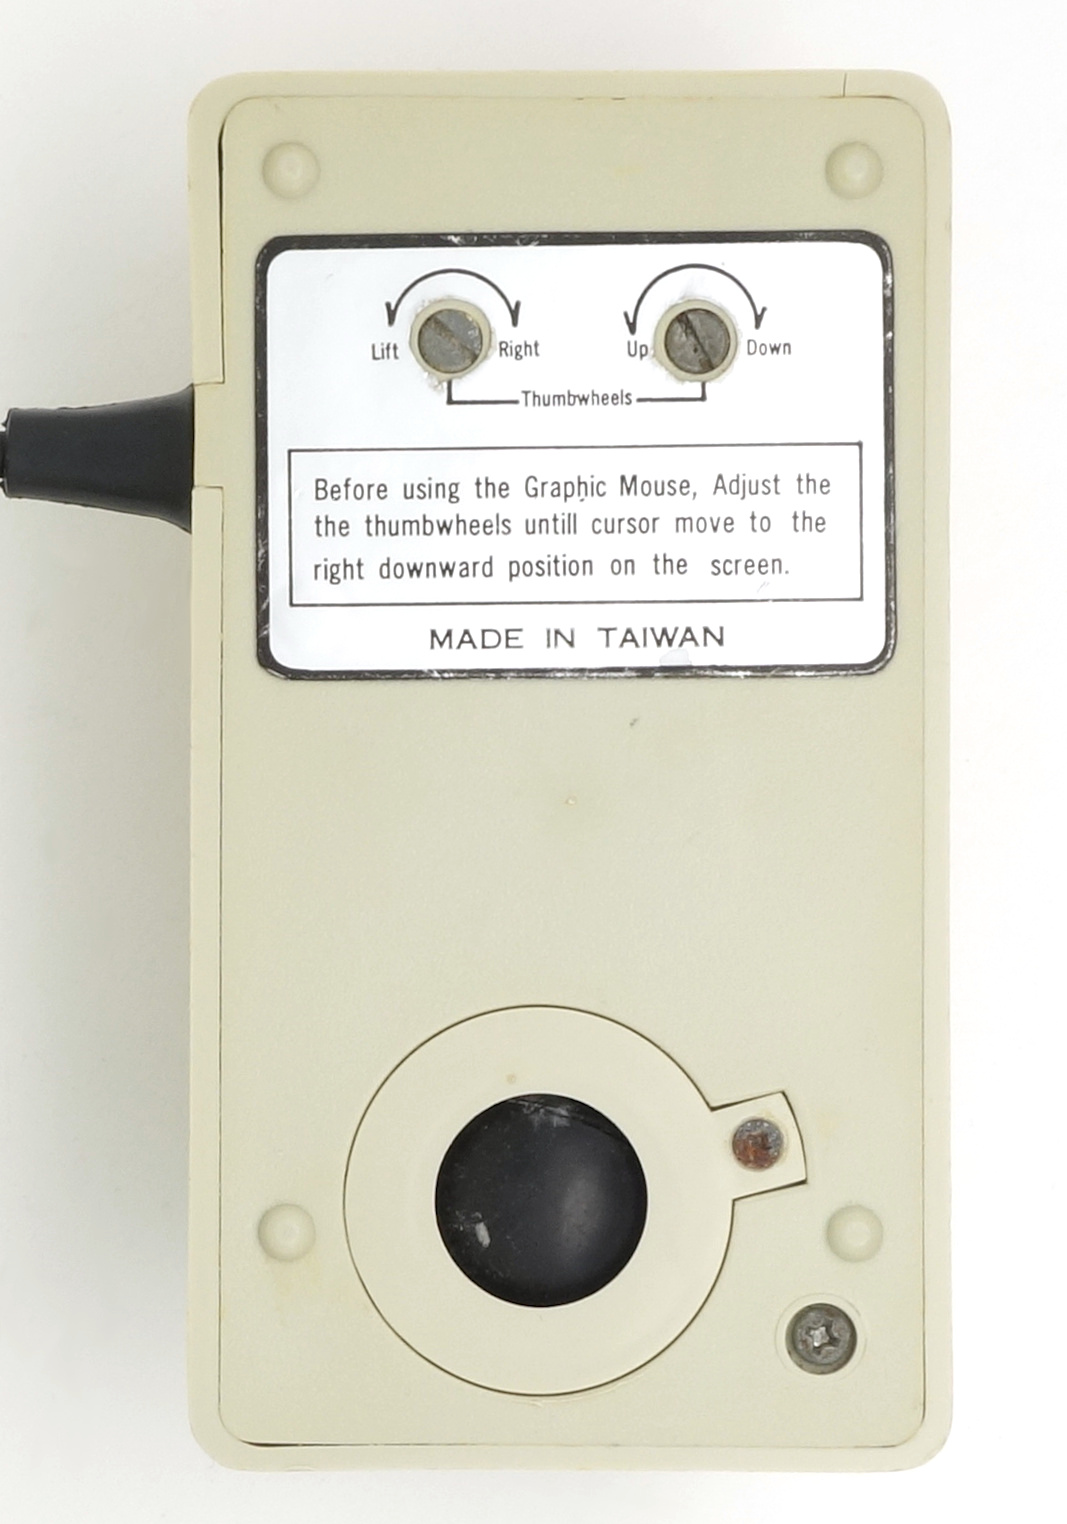
\includegraphics[scale=0.71]{1985_smc_contriver_magic_mouse/bottom_30.jpg}
    \caption{Magic Mouse, вид сверху и снизу}
    \label{fig:MagicMouseTopAndBottom}
\end{figure}

Цветовая дифференциация кнопок, очевидно, восходит к мышам Xerox для компьютеров Alto, в которых трем кнопкам были присвоены условные цветовые обозначения (документация Xerox использовала такие словосочетания, как <<красный щелчок мышью>> и <<желтый щелчок мышью>>, крайне неудачные с учетом того, что у большинства мышей для Alto кнопки в реальности оказывались одноцветными, выполненными из серого пластика). Мышь SMC для Commodore --- один из немногих манипуляторов, воплотивших эту цветовую дифференциацию в реальности. При этом вариант мыши для Apple II сделан иначе: он имеет красную левую кнопку и синие среднюю и правую (а пластик корпуса имеет более холодный серый оттенок).

\begin{figure}[h]
    \centering
    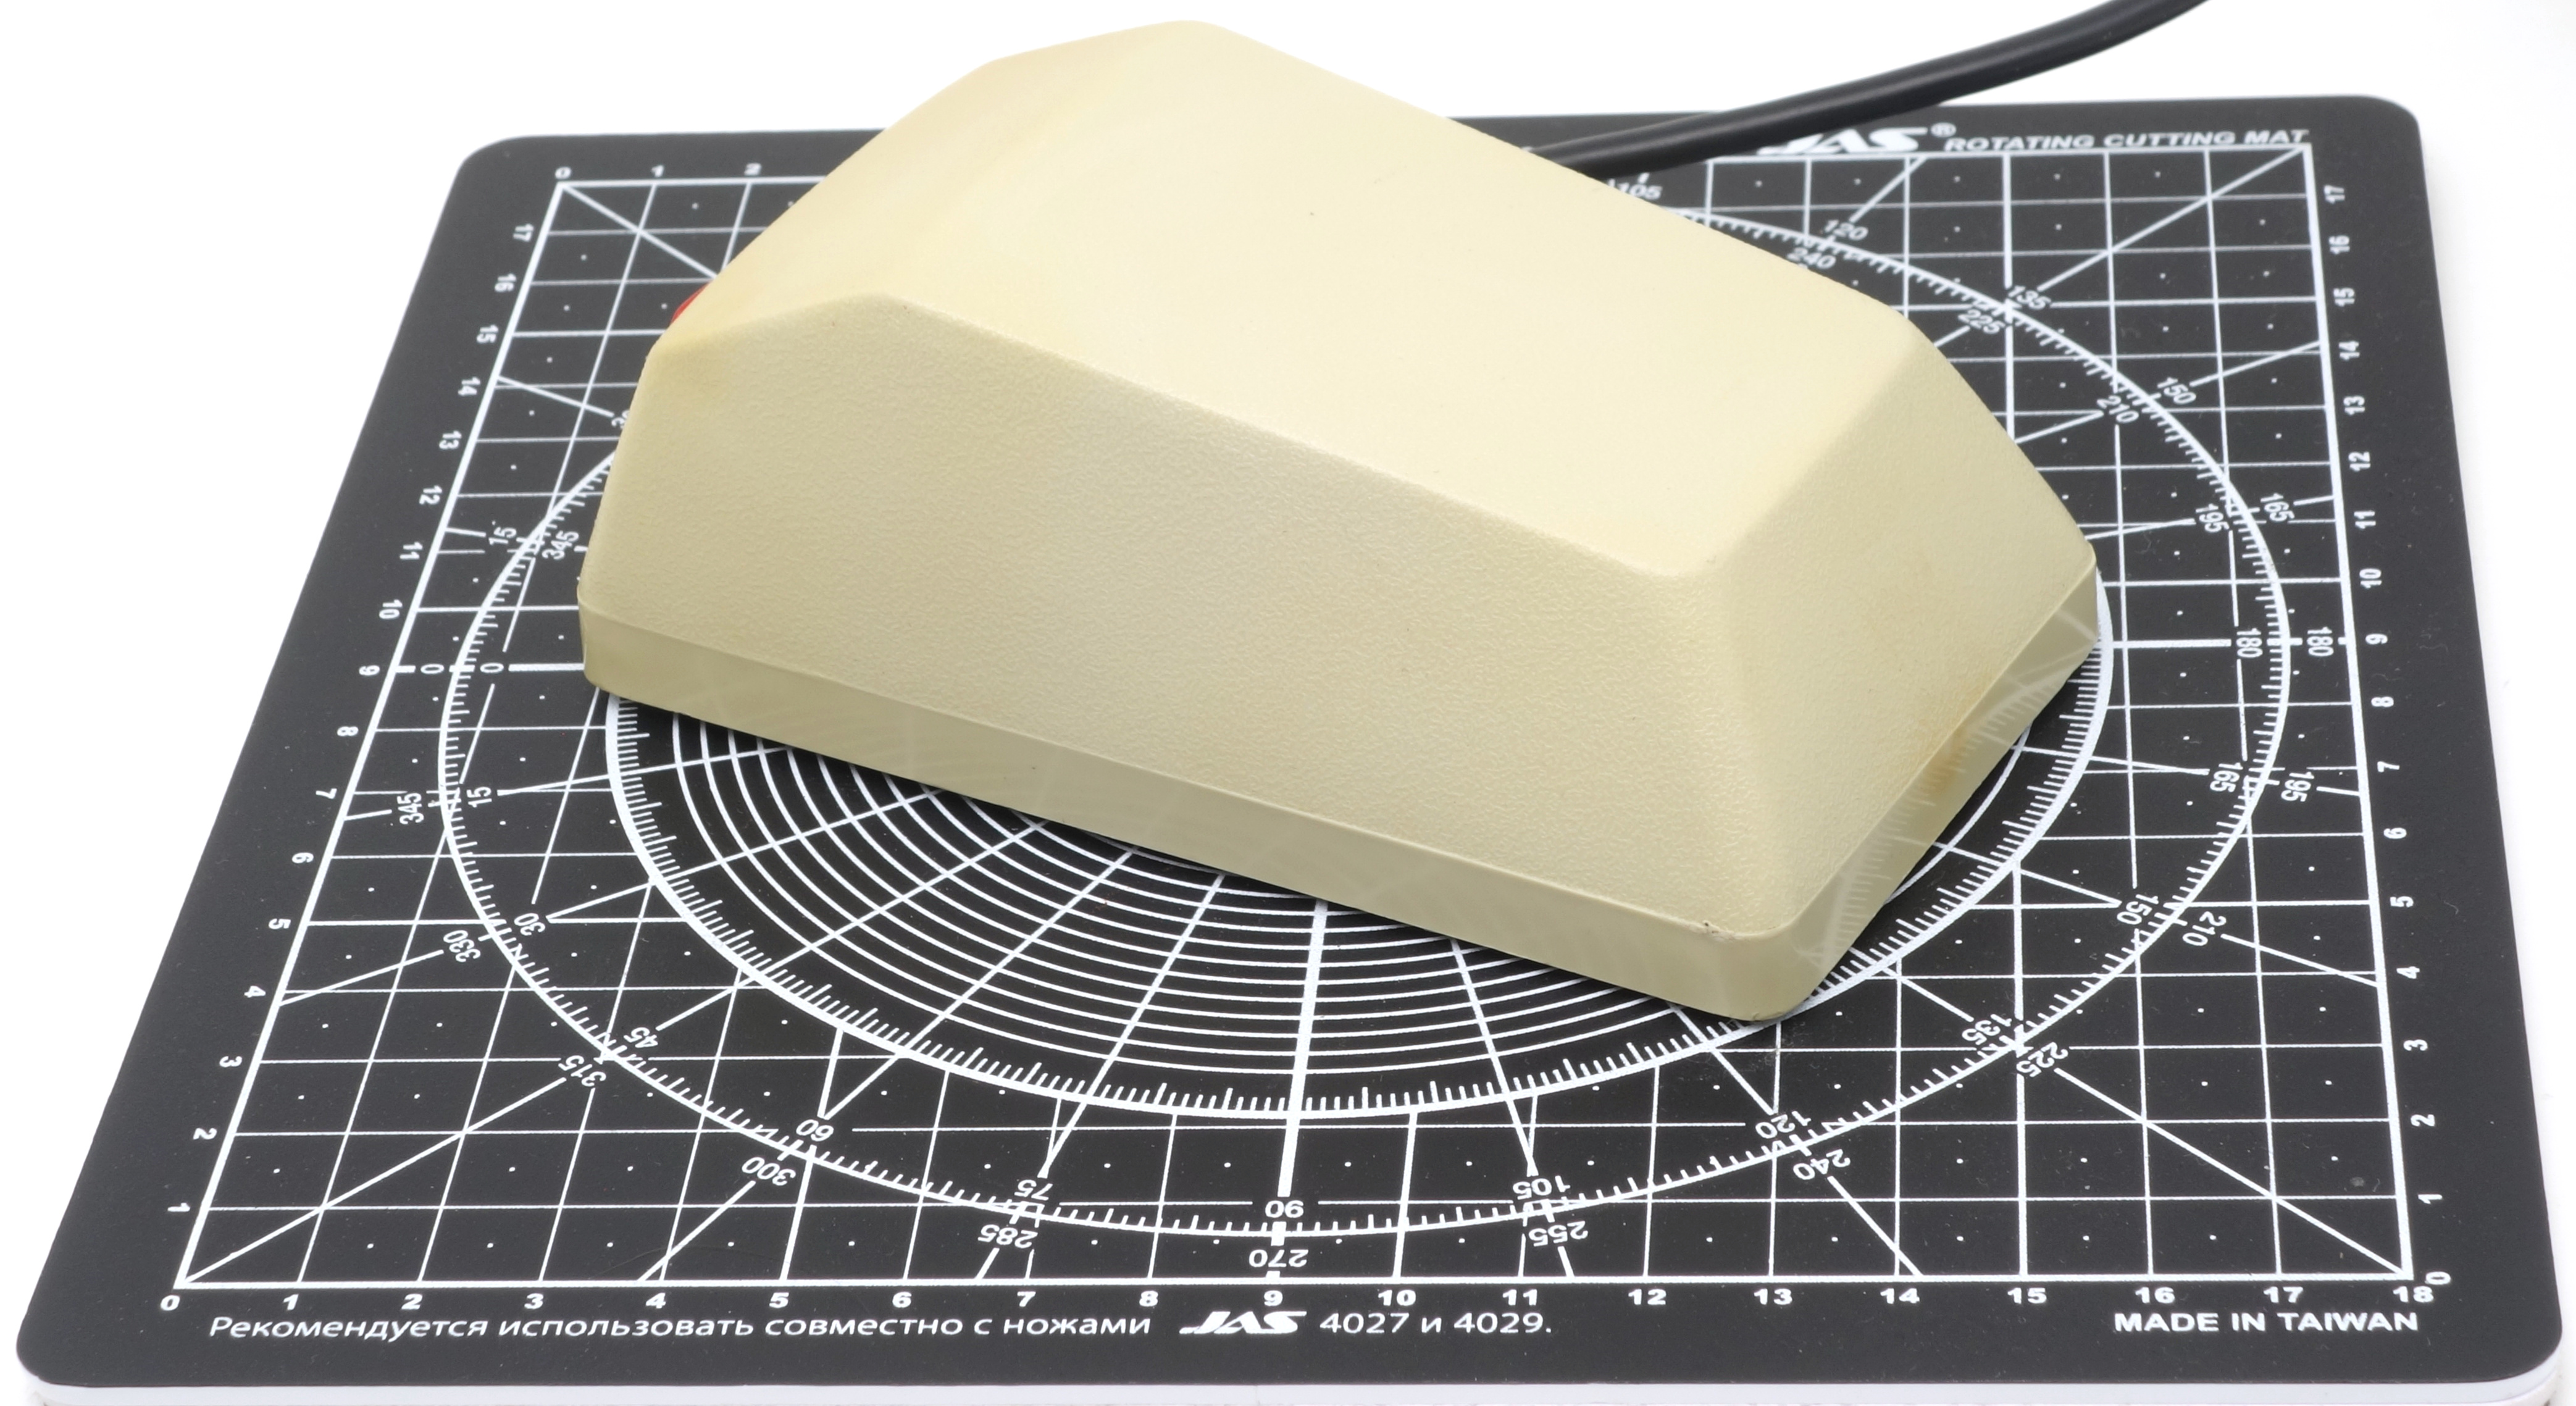
\includegraphics[scale=0.51]{1985_smc_contriver_magic_mouse/size_30.jpg}
    \caption{Magic Mouse на размерном коврике с шагом сетки 1~см}
    \label{fig:MagicMouseSize}
\end{figure}

Мышь является необычно крупной по меркам манипуляторов 80-х годов (рис. \ref{fig:MagicMouseSize}). Обозреватели отмечали это в качестве наиболее очевидного недостатка по сравнению с другими мышами, которые полностью помещаются под ладонью, наряду с большим весом мыши \cite{SMC_Mouse_Commodore3}.

Форма корпуса тоже признавалась в обзорах весьма неудобной. Неудачное расположение шара в зоне запястья пользователя (рис. \ref{fig:MagicMouseHand}) еще более затрудняло управление мышью. В дополнение, обозреватели отмечали дрожание курсора из-за неплотной посадки шара, а также низкого разрешения мыши, которое в прилагаемых к ней программах составляло всего $160 \times 200$ пикселей \cite{SMC_Mouse_Commodore3}. При этом ни один обозреватель не упоминал, что вертикальное расположение кнопок создает возможность при нажатии на них нечаянно сдвинуть мышь назад --- либо вероятность этого была сильно мала из-за веса и размеров мыши, либо этот недостаток оказывался несущественным на фоне остальных проблем ее аппаратного и программного обеспечения. В частности, в  \cite{SMC_Mouse_Commodore3} отмечается, что движения указателя отстают от перемещений мыши пользователем, и их позиции становятся синхронизированным только после прекращения движения, что сильно затрудняет точное позиционирование. Тонкая  работа с мышью оказалась крайне затруднена (помимо дребезга, ее осложняет и то, что фактическая нарисованная точка оказывается немного выше позиции указателя). Поэтому в идущем в коплекте с мышью графическом редакторе Hi-Res Graphic Designer для однопиксельного перемещения курсора в одном из восьми направлений используются клавиши клавиатуры.

\begin{figure}[h]
    \centering
    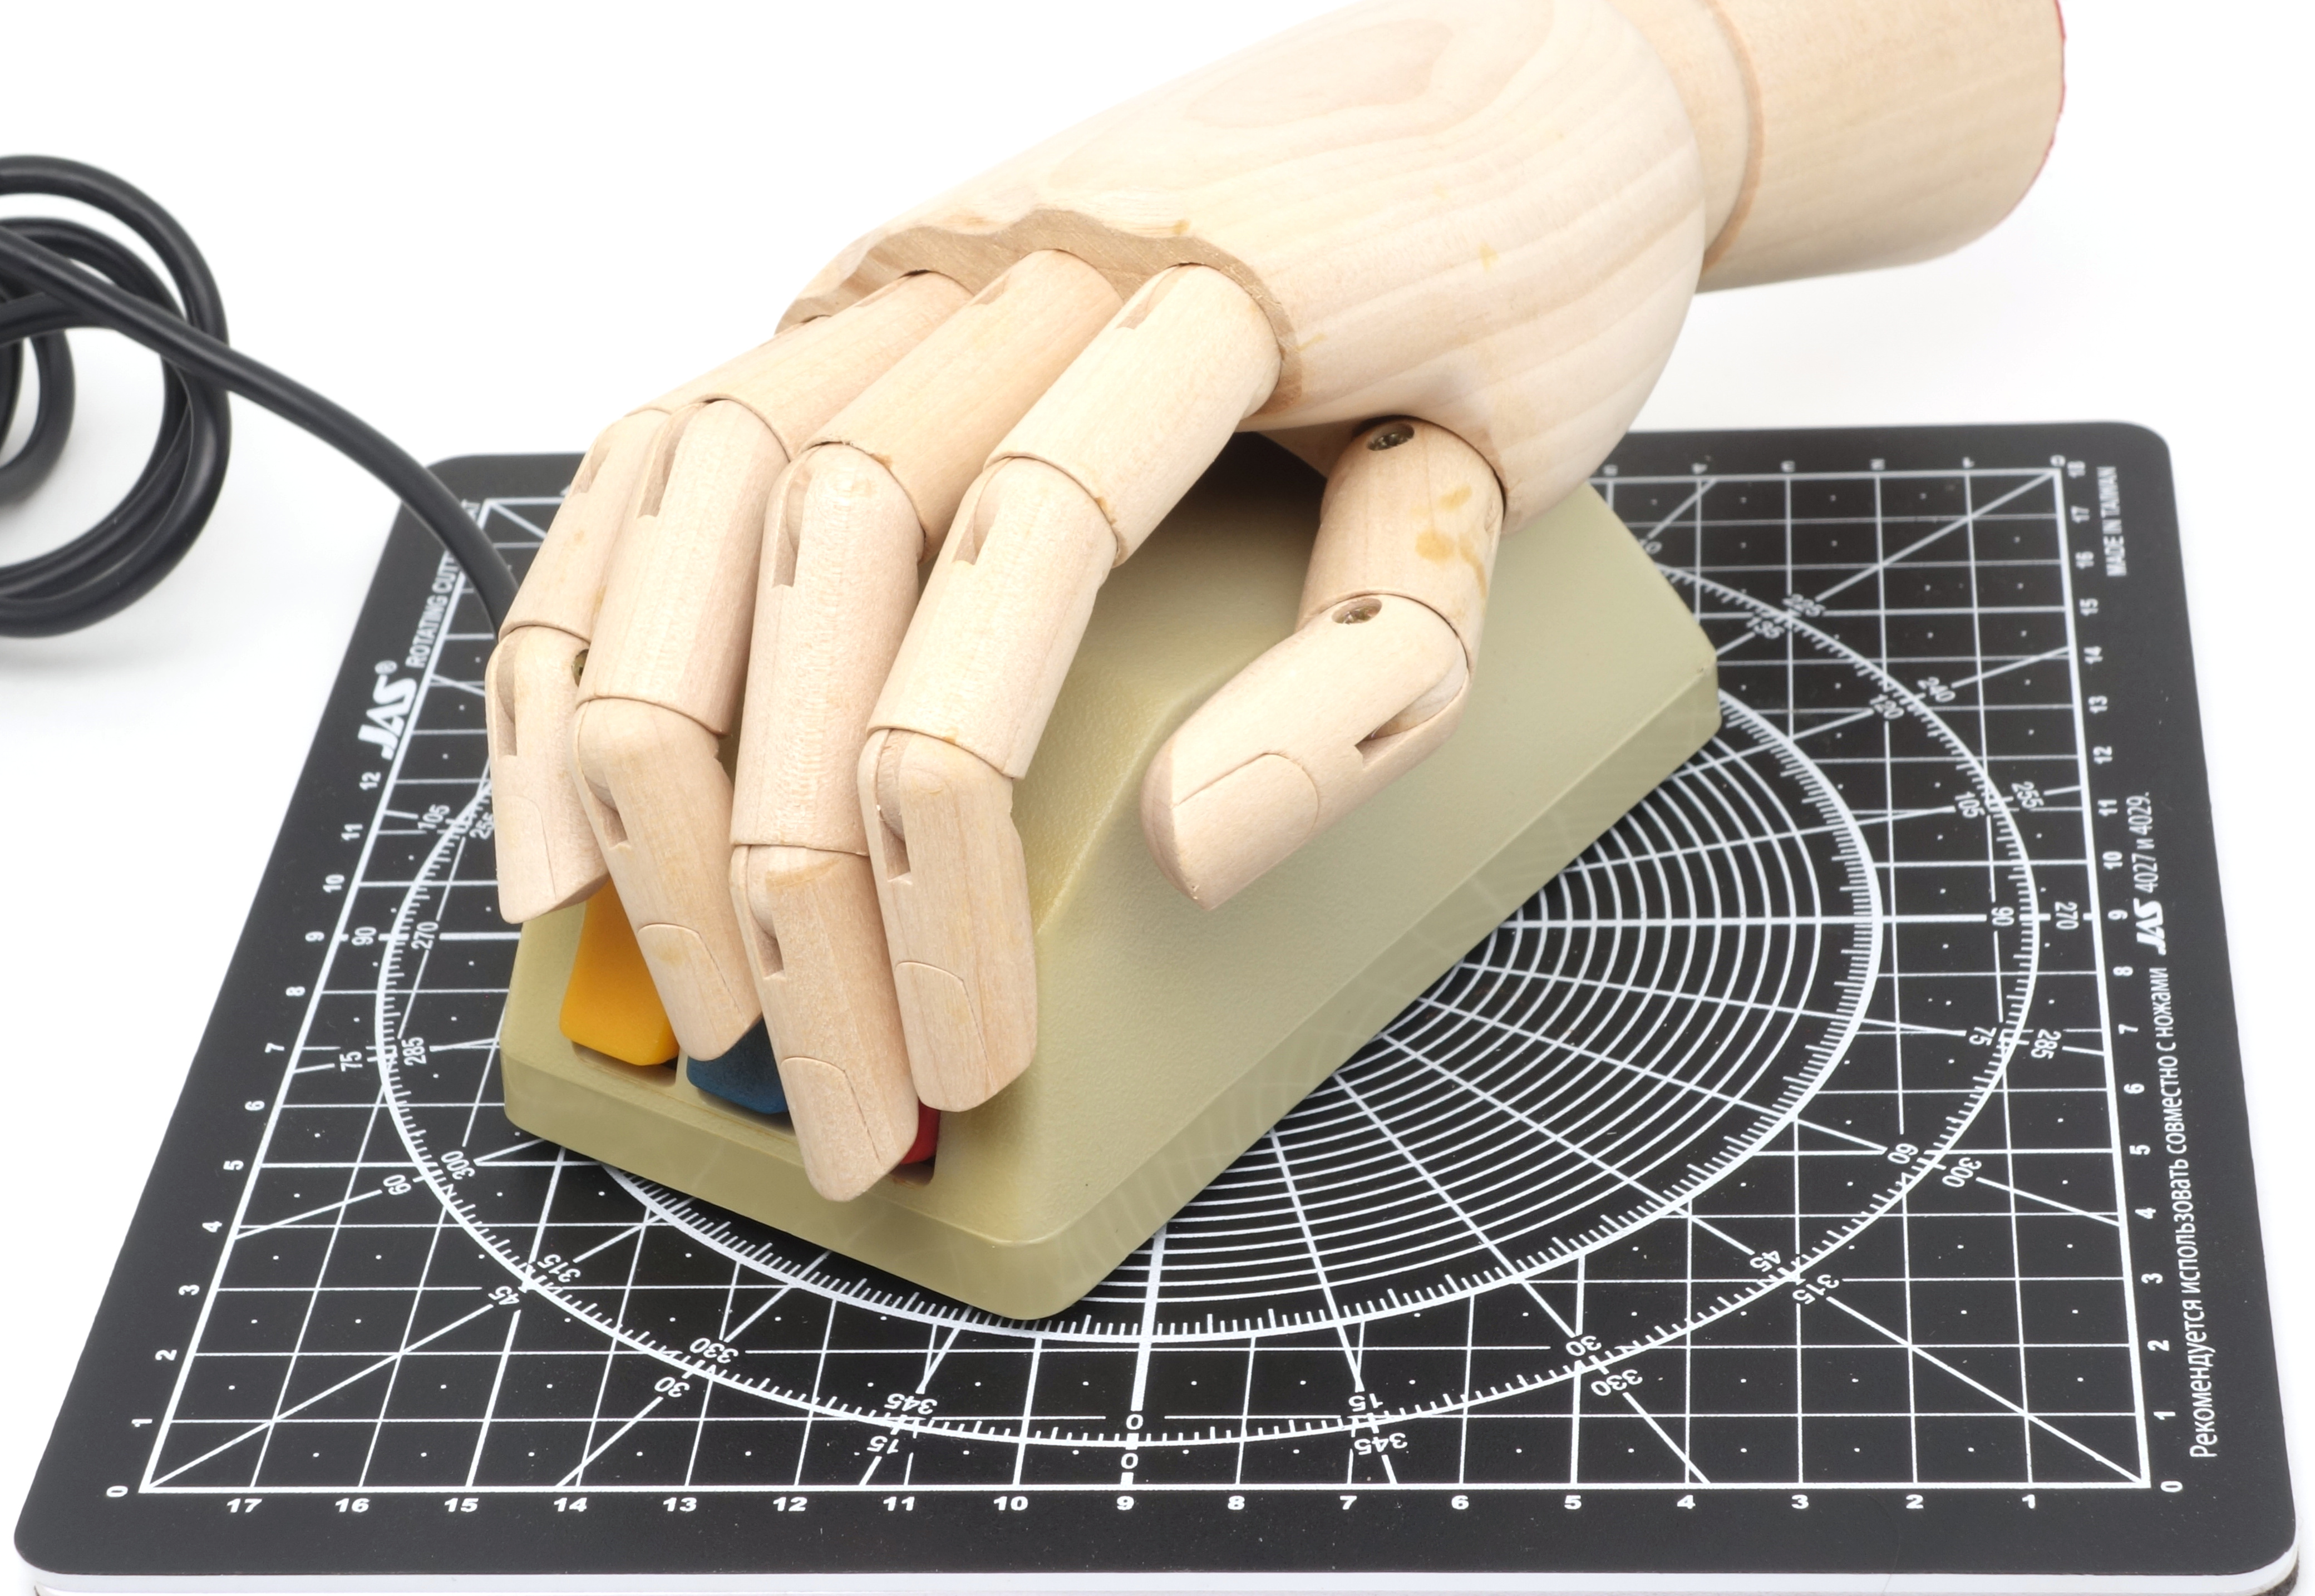
\includegraphics[scale=0.51]{1985_smc_contriver_magic_mouse/hand_30.jpg}
    \caption{Magic Mouse с моделью руки человека}
    \label{fig:MagicMouseHand}
\end{figure}

Неожиданным достоинством SMC Mouse была ее дешевизна: например, версия для компьютеров BBC Micro, несмотря на свои размеры и вес, стоила 59,95 фунтов стерлингов, в отличие от 89,95 фунтов стерлингов за стандартную для этих компьютеров мышь AMX первого поколения с аналогичной комплектацией. Очивидно, причиной была меньшая себестоимость за счет производства на Тайване, но также весьма вероятен и ценовой демпинг.

 \begin{figure}[h]
    \centering
    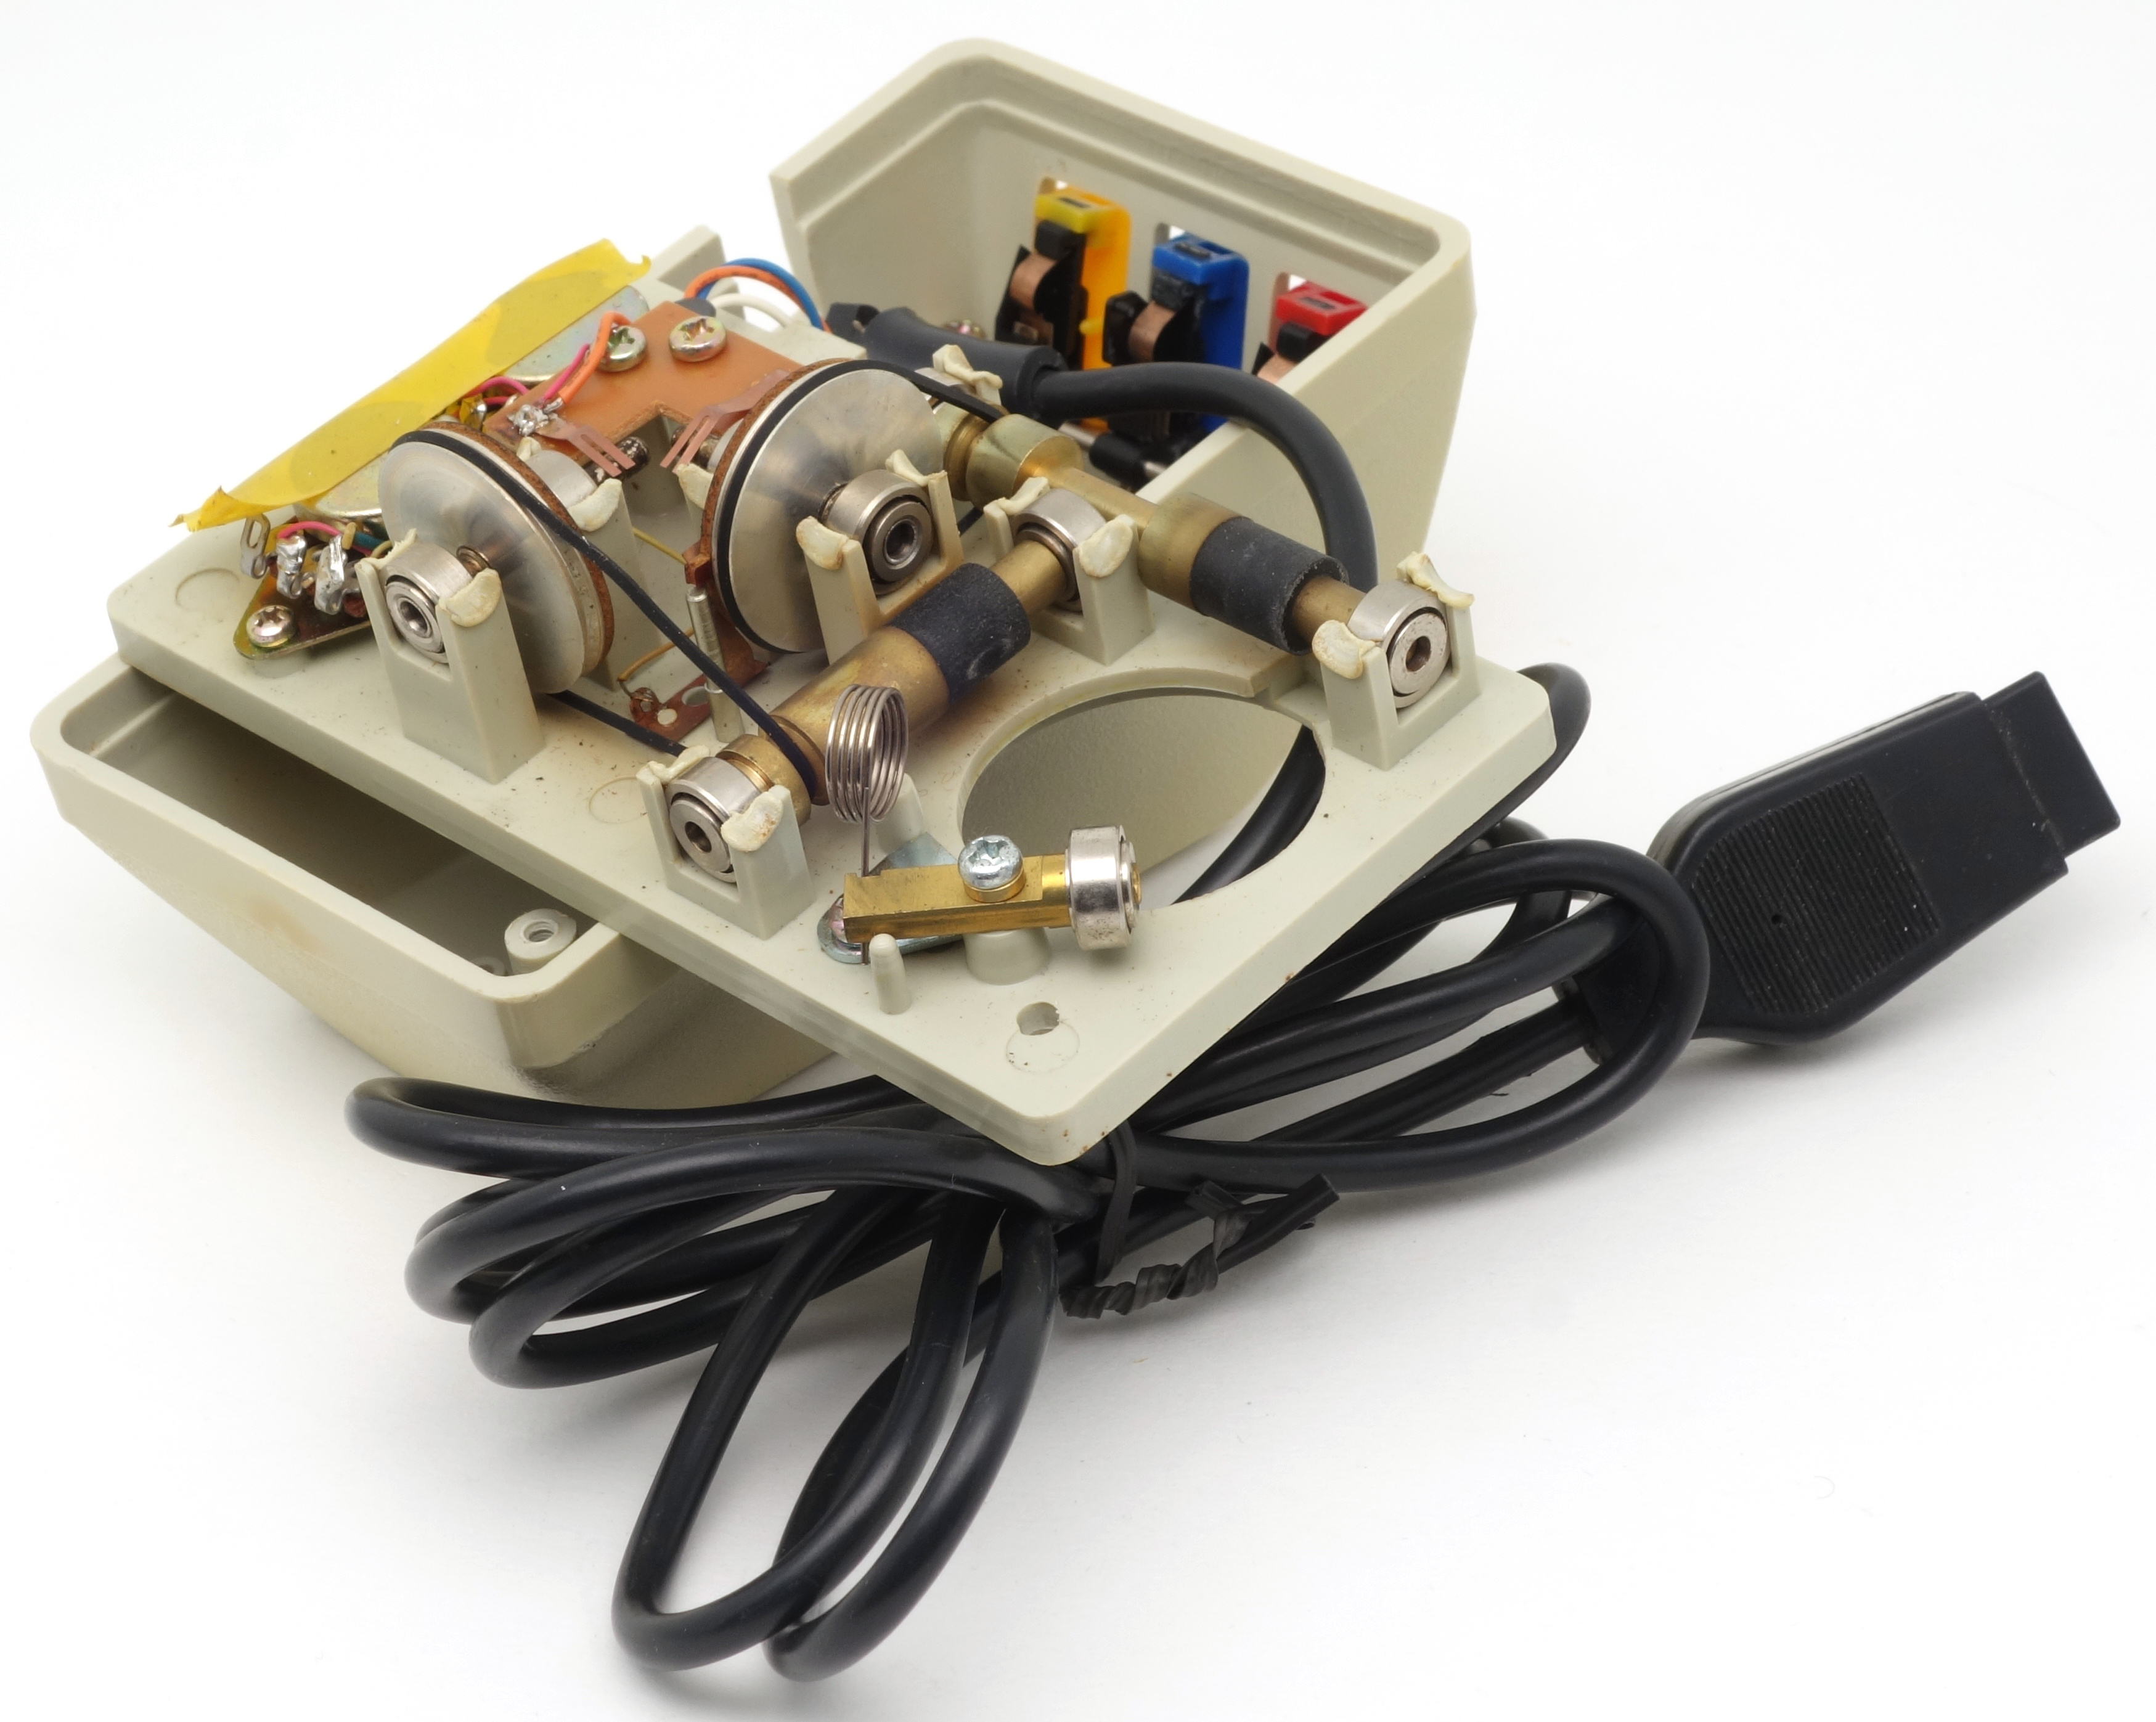
\includegraphics[scale=0.65]{1985_smc_contriver_magic_mouse/inside_30.jpg}
    \caption{Magic Mouse в разобранном виде}
    \label{fig:MagicMouseInside}
\end{figure}

Внутреннее устройство мыши показано на рисунке \ref{fig:MagicMouseInside}. Как можно видеть, вращение роликов шаром при перемещении мыши передается с помощью ременных передач на два потенциометра. В конструкции задействовано значительное число дорогих металлических деталей, оси роликов и потенциометры закреплены на подшипниках, что никак не соответствует дешевой отпускной цены изделия.

\begin{thebibliography}{9}
\bibitem{c64wiki} Mouse -- C64-Wiki \url{https://www.c64-wiki.com/wiki/Mouse}
\bibitem {SMC_Mouse_Commodore1} Mouse with graphics // Acorn user, June 1985. -- P. 127 \url{https://archive.org/details/AcornUser035-Jun85/page/n127/mode/2up}
\bibitem {SMC_Mouse_Commodore2} Connor P. Joysticks survey // Your computer, August, 1985. p. 32--34 \url{https://archive.org/details/your-computer-magazine-1985-08/page/n33/mode/2up}
\bibitem {SMC_Mouse_Commodore3} Janda D. Hardware pro-test: SMC Mouse // Personal Computer News, Iss. 107, April 20, 1985. -- P. 32 \url{https://archive.org/details/PersonalComputerNews/PersonalComputerNews107-20Apr1985/page/n33/mode/2up}
\bibitem {CHM} Ideal Magic Mouse. Computer History Museum. \url{https://www.computerhistory.org/collections/catalog/102633276}
\bibitem {reddit} Mice. (and a story!). reddit.com
 \url{https://www.reddit.com/r/retrobattlestations/comments/8ket13/mice_and_a_story/}
\end{thebibliography}
\end{document}
